% Chapter 3

\chapter{Methodology}\label{Chapter3}

%----------------------------------------------------------------------------------------

\section{Data Description}

This study draws on a clinical neuropsychological database maintained by a neurorehabilitation service. The raw extraction contains 22,075 records from 8,739 distinct patients, including longitudinal follow-up assessments. Each assessment comprises 31 variables spanning demographic and administrative information, injury characteristics, and neuropsychological measures across six cognitive domains: orientation, attention, visuoperception, language, memory, and executive function. After the Tier-1 filtering described in Section~\ref{sec:filtering}, the analysed dataset contains 17{,}406 assessments from 7{,}285 patients.

The data were generated in routine clinical care, not under a fixed research protocol. Test selection was determined by the neuropsychologist, the referral question, and the patient's capacity to engage with the battery. Missingness is therefore structured. Some measures are present in nearly every assessment; others appear only in particular clinical contexts. Unlike research-protocol missingness, which is often controlled by design, missingness in this dataset ranges from below 5\% for screening measures to above 90\% for specialised tests.

The measures also occupy different scales, including standardised $z$-scores, scaled scores, and raw timed variables. These scales were harmonised during domain aggregation (Section~\ref{sec:domain_scores}). Table~\ref{tab:missing_descriptive} reports the missingness pattern for the 14 eligible variables. Only 53.1\% of the 17,406 records (9,245 assessments) are complete across all 14 variables; listwise deletion would remove 46.9\% of the sample and risk substantial selection bias. The imputation strategy in Section~\ref{sec:imputation} is designed to avoid that loss of clinical information. All data were anonymised according to institutional governance standards.

%----------------------------------------------------------------------------------------

\section{Tier 1 Filtering}\label{sec:filtering}

Because several variables contain substantial missingness, filtering was applied before imputation and clustering. The main analysis uses a 50\% threshold. Variables missing in more than half of the observations are removed, and observations with more than 50\% missingness across retained variables are also excluded.

The threshold balances coverage against reliability. A 70\% threshold would preserve more records and variables, but at the cost of heavier imputation and greater risk of artefactual structure. A 30\% threshold would yield a cleaner matrix but would discard clinically informative assessments and reduce statistical power. The 50\% rule retains a broad cross-section of cognitive domains while constraining the burden placed on imputation. Sensitivity analyses across thresholds from 30\% to 70\% are reported in Section~\ref{sec:robustness}.

After applying this cut-off and removing assessments with no cognitive test on file, the final dataset contains 14 neuropsychological variables and 17,406 assessments from 7,285 patients.

\begin{table}[ht]
\caption{Eligible neuropsychological variables after Tier~1 filtering, organised by cognitive domain.}
\label{tab:eligible_vars}
\centering
\small
\begin{tabular}{l p{0.55\textwidth} c}
\toprule
\textbf{Cognitive Domain} & \textbf{Variables} & \textbf{Count} \\
\midrule
Orientation        & \texttt{OPERSONA}, \texttt{OESPAI}, \texttt{OTEMPS} & 3 \\
Attention          & \texttt{ASPAN}, \texttt{ATMTA} & 2 \\
Visuoperception    & \texttt{VPIMATGES} & 1 \\
Language           & \texttt{LREPETICIOTB}, \texttt{LDENOMINACIOTB}, \texttt{LCOMPRENSIOTB} & 3 \\
Memory             & \texttt{MDIGITS}, \texttt{MRAVLT075}, \texttt{MRAVLT015}, \texttt{MRAVLT015R} & 4 \\
Executive Function & \texttt{FEPMR} & 1 \\
\midrule
\textbf{Total}     & & \textbf{14} \\
\bottomrule
\end{tabular}
\end{table}

%----------------------------------------------------------------------------------------

\section{Imputation Methods}\label{sec:imputation}

I implemented a comparative framework with ten imputation methods across five categories, extending the taxonomy of \textcite{afkanpour2024identify} to include deep learning. Chapter~\ref{Chapter2}, §\ref{sec:lit_imputation}, explains the rationale for each method. Table~\ref{tab:method_summary} summarises each method's category, year, main trade-offs, and downstream clustering performance. Hyperparameters are listed in Appendix~\ref{AppendixA}, Table~\ref{tab:imputation_hyperparams}. The two deep-learning methods are described in more detail here because their training schedules require additional design choices.

\noindent \textbf{DAE.} As a denoising autoencoder, this model is designed to reconstruct complete data from deliberately corrupted inputs. Under a \textit{missingness-pattern-aware} corruption scheme, the input is masked via $\tilde{x}_{ij}=m_{ij}\,x_{ij}$. To ensure a diversity of regularisation, half the training samples are given uniform corruption, while for the other half the mask $\mathbf{m}_i$ is drawn from the empirical co-occurrence distribution of missing-data patterns:
\begin{equation}\label{eq:dae_corrupt}
\mathbf{m}_i\sim
\begin{cases}
P_{\mathrm{miss}} & \text{with probability } 0.5,\\[2pt]
\operatorname{Bernoulli}(1-\rho)^{\otimes p} & \text{with probability } 0.5,
\end{cases}
\end{equation}
Here $P_{\mathrm{miss}}$ is the observed missingness pattern in the data and $\rho$ is the rate of uniform corruption. This matters because missingness in clinical data has structure: some tests are absent together because they belong to the same sub-battery or place similar demands on the patient. By training the DAE on corruption patterns that resemble clinical missingness, the model is encouraged to learn inter-variable dependencies relevant to the latent cognitive structure.

\noindent \textbf{VAE.} I use a variational autoencoder with an ELBO (Eq.~\ref{eq:vae}) that combines MSE on the observed entries with a Kullback--Leibler divergence term, weighted by $\beta$, to regularise the latent distribution toward a standard Gaussian prior. Keeping $\beta$ fixed can lead to posterior collapse, where the model ignores the latent variables and relies mainly on the decoder. To reduce this risk, I use cyclical annealing, which increases $\beta$ up to $\beta_{\max}$ over a cycle of $T$ epochs before resetting it:
\begin{equation}\label{eq:beta_cyclical}
\beta(t)=\beta_{\max}\,\frac{t \bmod T}{T},\qquad T=40,\ \beta_{\max}=0.1,
\end{equation}
This schedule alternates between emphasising reconstruction (low $\beta$) and regularising the latent space (high $\beta$).

To evaluate the two deep-learning methods, I performed a held-out evaluation across three folds. In each case I set aside 10 per cent of the observed values in a set $H$, retrained, and then computed the RMSE and MAE between the imputed and actual figures:
\begin{equation}\label{eq:rmse}
\mathrm{RMSE}=\sqrt{\frac{1}{|H|}\sum_{(i,j)\in H}\bigl(\hat{x}_{ij}-x_{ij}\bigr)^2},\qquad
\mathrm{MAE}=\frac{1}{|H|}\sum_{(i,j)\in H}\bigl|\hat{x}_{ij}-x_{ij}\bigr|.
\end{equation}

\begin{table}[htbp]
\caption{A summary of the ten imputation methods broken down by the five-category taxonomy. For clustering performance (silhouette score and number of clusters $k$) I took the best UMAP+HDBSCAN solution on the domain-level features. Note that the silhouette is on the high-density core that HDBSCAN clusters directly (before the $k$-nearest-neighbour noise-reassignment step), so it runs slightly above the final full-coverage silhouette quoted in the text (for instance MICE scores 0.598 on the core and 0.526 once every assessment is assigned; see §\ref{sec:h1_results}).}
\label{tab:method_summary}
\centering
\scriptsize
\renewcommand{\arraystretch}{1.4}
\begin{tabular}{@{} p{1.8cm} l c c c p{3.2cm} p{3cm} @{}}
\toprule
\textbf{Category} & \textbf{Method} & \textbf{Year} & \textbf{$k$} & \textbf{Sil.} & \textbf{Advantages} & \textbf{Limitations} \\
\midrule
Conventional & Mean       & ---  & 4 & 0.604 & Simplest; fast; universal baseline & Collapses variance \& covariance \\
Statistical  & EM         & 1977 & 4 & 0.587 & Principled MLE; preserves covariance & Assumes multivariate normality \\
             & MICE       & 2011 & 3 & 0.598 & Flexible; preserves distribution & Requires model per variable \\
\midrule
Machine      & KNN        & 2001 & 4 & 0.576 & Non-parametric; captures local structure & Sensitive to $k$; slow for large $n$ \\
Learning     & MissForest & 2012 & 3 & 0.606 & Non-linear; handles mixed types & Computationally expensive \\
\midrule
Hybrid       & PMM        & ---  & 4 & 0.498 & Preserves marginal distribution & Requires adequate donor pool \\
\midrule
Matrix       & SoftImpute & 2010 & 4 & 0.571 & Efficient for sparse matrices & Assumes low-rank structure \\
Completion   & NMF        & 1999 & 3 & 0.546 & Non-negativity natural for scores & Sensitive to rank choice \\
\midrule
Deep         & DAE        & 2018 & 5 & 0.510 & Non-linear; multiple imputations & Requires hyperparameter tuning \\
Learning     & VAE        & 2014 & 4 & 0.603 & Probabilistic; principled uncertainty & Complex training; $\beta$-tuning \\
\bottomrule
\end{tabular}

\vspace{0.5em}
\raggedright
\scriptsize
\textit{References:} Mean \parencite{little2019statistical}; PMM \parencite{vanbuuren2011mice}; EM \parencite{dempster1977maximum}; MICE \parencite{vanbuuren2011mice}; KNN \parencite{troyanskaya2001missing}; MissForest \parencite{stekhoven2012missforest}; SoftImpute \parencite{mazumder2010spectral}; NMF \parencite{lee1999learning}; DAE \parencite{gondara2018mida}; VAE \parencite{kingma2014auto, mccoy2018variational}.
\end{table}

%----------------------------------------------------------------------------------------

\section{Domain Score Computation}\label{sec:domain_scores}

Domain-level features were constructed by aggregating variables within each cognitive domain while retaining the 14 individual neuropsychological variables for comparison. Because the original measures combine standardised scores, scaled scores, and raw timed variables such as the Trail Making Test, aggregation without scale harmonisation would be inappropriate. A timed measure with a wide numerical range could otherwise dominate a composite for purely metric reasons.

Three preprocessing operations were applied before aggregation. Each variable was winsorised to the 1st--99th percentile to limit the influence of implausible imputed extremes or sentinel codes. Timed tests were sign-reversed so that higher values consistently denoted better performance. All variables were then $z$-standardised to zero mean and unit variance. Domain scores were computed as reliability-weighted averages, with each variable assigned weight $w_j = 1 - r_j$, where $r_j$ is its missingness rate; weights were normalised within domain. Tests administered more frequently therefore contribute more strongly to the corresponding composite. The resulting representation reduces the 14-variable space to six domain scores: orientation, attention, visuoperception, language, memory, and executive function.

This aggregation is methodologically useful but not cost-free. Composite scores tend to be more reliable than single tests because averaging reduces random measurement error, and reducing dimensionality from 14 variables to 6 domains improves the geometry available to distance-based algorithms. Domain-level profiles are also closer to clinical interpretation, since neuropsychologists usually reason about cognitive domains rather than isolated variables. Detail is inevitably lost. Two patients may share the same average memory score while differing in immediate versus delayed recall. Hypothesis~H4 tests whether the gains in stability and interpretability justify that compression.

%----------------------------------------------------------------------------------------

\section{UMAP + HDBSCAN Pipeline}\label{sec:pipeline}

Figure~\ref{fig:pipeline_diagram} summarises the pipeline from imputed data to final cluster assignment.

\begin{figure}[htbp]
\centering
\resizebox{\textwidth}{!}{%
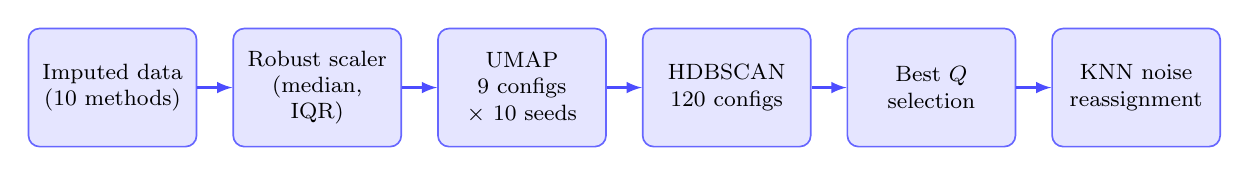
\begin{tikzpicture}[
  box/.style={draw=blue!60, line width=0.6pt, rounded corners,
              fill=blue!10, text width=1.9cm, minimum height=1.5cm,
              align=center, font=\footnotesize},
  arr/.style={->, line width=0.9pt, draw=blue!70, >=latex}
]
  \node[box] (imp) at (0,0)    {Imputed data\\(10 methods)};
  \node[box] (std) at (2.6,0)  {Robust scaler\\(median, IQR)};
  \node[box] (umap) at (5.2,0) {UMAP\\9 configs\\$\times$ 10 seeds};
  \node[box] (hdb) at (7.8,0)  {HDBSCAN\\120 configs};
  \node[box] (sel) at (10.4,0) {Best $Q$\\selection};
  \node[box] (knn) at (13.0,0) {KNN noise\\reassignment};
  \draw[arr] (imp) -- (std);
  \draw[arr] (std) -- (umap);
  \draw[arr] (umap) -- (hdb);
  \draw[arr] (hdb) -- (sel);
  \draw[arr] (sel) -- (knn);
\end{tikzpicture}%
}
\caption[Pipeline overview]{End-to-end clustering pipeline. After imputed data are run through a robust scaler, they go into a UMAP hyperparameter grid (10 random seeds for each of 9 configurations) and the embedding with the best silhouette is kept. HDBSCAN then does the clustering in a 120-configuration sweep, scored by the composite quality criterion $Q = \text{silhouette} \times (1 - \text{noise fraction})$, with any boundary noise points re-assigned via $k$-nearest-neighbour. The whole thing runs on each of the 10 imputation outputs.}
\label{fig:pipeline_diagram}
\end{figure}

Before dimensionality reduction, features are scaled with the median and interquartile range. Robust scaling is appropriate here because neuropsychological data often exhibit floor and ceiling effects \parencite{bellio2020analyzing}. Severely impaired patients may accumulate at the minimum, while intact patients may accumulate near the maximum; both patterns can distort means and standard deviations \parencite{pinsky2023mad}. Median and interquartile-range scaling reduce this influence.

For each of the 20 imputed datasets (10 methods across 2 feature representations), UMAP is applied before HDBSCAN. UMAP is stochastic, so a single embedding can reflect random initialisation as well as data geometry. I therefore run 10 seeds for each hyperparameter set and retain the embedding with the highest silhouette score under an initial HDBSCAN evaluation. This repeated-seed procedure constrains seed-specific variation without changing the downstream clustering logic.

\subsection{UMAP Parameter Grid}

\begin{table}[ht]
\caption{UMAP hyperparameter grid. All combinations of these values were put through their paces, for a total of 9 configurations.}
\label{tab:umap_grid}
\centering
\begin{tabular}{l l}
\toprule
\textbf{Parameter} & \textbf{Values} \\
\midrule
\texttt{n\_neighbors}  & 15, 30, 50 \\
\texttt{min\_dist}     & 0.0 \\
\texttt{n\_components} & 3, 5, 8 \\
\bottomrule
\end{tabular}
\end{table}

The Euclidean metric was used, and \texttt{min\_dist} was set to 0.0 to encourage separation between dense regions in the embedding.

\subsection{HDBSCAN Parameter Grid}

\begin{table}[ht]
\caption{HDBSCAN hyperparameter grid. All listed value combinations were evaluated, giving me 120 configurations for each UMAP embedding.}
\label{tab:hdbscan_grid}
\centering
\begin{tabular}{l l}
\toprule
\textbf{Parameter} & \textbf{Values} \\
\midrule
\texttt{min\_cluster\_size}          & 500, 1000, 1500, 2000, 3000 \\
\texttt{min\_samples}                & 5, 10, 25, 50 \\
\texttt{cluster\_selection\_method}  & eom, leaf \\
\texttt{cluster\_selection\_epsilon} & 0.0, 0.1, 0.5 \\
\bottomrule
\end{tabular}
\end{table}

All 120 HDBSCAN configurations were evaluated for every UMAP configuration, giving $9 \times 120 = 1{,}080$ candidate solutions per dataset. To select the best configuration, I used a composite quality score that penalises solutions that achieve a high silhouette by assigning too many observations to noise:
\begin{equation}
Q = \text{silhouette} \times (1 - \text{noise proportion})
\label{eq:quality}
\end{equation}

\subsection{Sweep Procedure}

For each imputed dataset, the procedure was as follows. First, I standardised the features with the robust scaler. Second, I generated ten embeddings for each of the nine UMAP configurations and retained the best embedding as the reference UMAP representation. Third, I applied all 120 HDBSCAN configurations and selected the one with the highest $Q$ score. Finally, I reassigned any observations labelled as noise.

During reassignment, HDBSCAN noise points are allocated to the nearest substantive cluster using $k$-nearest neighbours ($k=10$) in UMAP space. Because residual noise is minimal on these features, this step produces 100\% coverage, so every assessment receives a cluster label. Reassignment is accepted only if the silhouette score does not fall by more than 10\%, preserving the separation of the clusters.

\subsection{Worked Example}

Consider a hypothetical patient who completed the orientation and digit span tasks but did not complete the Trail Making Test because of motor impairment or the Rey Auditory Verbal Learning delayed recall because of fatigue. After Tier~1 filtering, the patient remains in the dataset with the eligible variables, and MICE imputes the two missing scores from the observed information.

The 14 variable-level scores are then winsorised, direction-aligned, standardised, and reliability-weighted as described in Section~\ref{sec:domain_scores}, producing six domain composites. The robust scaler is applied to reduce the impact of floor and ceiling effects. The resulting six-dimensional vector is mapped into the cohort's UMAP embedding. HDBSCAN assigns the patient to one of three cognitive-severity tiers: Above-Average, Near-Normal, or Global Impairment. If the patient lies in a low-density boundary region and is labelled as noise, the KNN reassignment step uses the ten closest assessments in the embedding to assign the nearest substantive tier. The final output is a tier label and, under the H2 consensus procedure, a confidence score showing how often the imputation methods agree.

%----------------------------------------------------------------------------------------

\section{Hypothesis Definitions}\label{sec:hypotheses}

\noindent \textbf{H1 (Existence of Cognitive Clusters).} The UMAP + HDBSCAN pipeline is expected to identify at least two separate, stable cognitive clusters for most imputation methods. H1 is supported if the best solution from at least eight of the ten methods satisfies both criteria: mean silhouette $\ge 0.40$, indicating adequate separation and cohesion, and noise proportion $< 0.30$, indicating that most observations are assigned to substantive clusters. The 80\% criterion allows limited method-specific failure without rejecting the overall hypothesis.

\noindent \textbf{H2 (Robustness Across Imputation Methods).} Cluster solutions should show moderate to high agreement across imputation methods. H2 is supported if the median pairwise ARI and NMI across all $\binom{10}{2} = 45$ method pairs exceed 0.50. This threshold is above chance and indicates substantial membership overlap, without requiring exact identity across solutions.

\noindent \textbf{H3 (Association with Clinical Unit).} Cluster membership is expected to be associated with clinical unit. For each imputation method, a contingency table is constructed and a chi-square test of independence is applied. H3 is supported if the association remains significant at $\alpha = 0.05$ after Bonferroni correction and Cram\'{e}r's V exceeds 0.10. A Cochran-Mantel-Haenszel (CMH) test, stratified by an appropriate covariate, is used as a sensitivity check for confounding.

\noindent \textbf{H4 (Domain-Level vs.\ Variable-Level Clustering).} I expect domain-level features to produce a clustering representation that is easier to interpret and at least as well separated as the variable-level representation. H4 is considered supported if the domain-level approach outperforms the variable-level approach on at least two of three measures: a higher silhouette score, a lower mean variance inflation factor (VIF), and a lower condition number. Lower VIF and condition number values indicate less multicollinearity and better numerical conditioning. Cross-method agreement is not used for H4 because it is already evaluated under H2; this comparison focuses only on feature representation.

%----------------------------------------------------------------------------------------

\section{Statistical Tests and Validation}\label{sec:stats}

\subsection{Statistical Conventions}

The inferential analysis follows standard statistical practice. Each test evaluates the data against a null hypothesis ($H_0$), which represents the no-effect baseline. The $p$-value is the probability of observing a test statistic as extreme as the one obtained, assuming $H_0$ is true; smaller values provide stronger evidence against $H_0$. A significance level of $\alpha = 0.05$ is pre-registered as the rejection threshold. For any parameter, a 95\% confidence interval represents the range that would contain the true value in 95\% of repeated samples under the same procedure.

When bootstrap methods are used, the observed data are resampled with replacement to approximate the sampling distribution of a statistic. The 2.5th and 97.5th percentiles of that empirical distribution form the bootstrap confidence interval. A $z$-score expresses a value in standard deviations from the mean of a reference distribution. For the neuropsychological tests used here, standardisation against normative populations allows scores to be compared across instruments.

Effect sizes follow Cohen's conventions. The standardised mean difference, Cohen's $d$, is calculated as
\begin{equation}\label{eq:cohend}
d=\frac{\bar{x}_1-\bar{x}_2}{s_p},\qquad s_p=\sqrt{\frac{(n_1-1)s_1^2+(n_2-1)s_2^2}{n_1+n_2-2}},
\end{equation}
with $s_p$ being the pooled standard deviation. By this measure, $d=0.2$ is small, $0.5$ medium, and $0.8$ large. In the case of Cram\'{e}r's V as an effect size for chi-squared tests (Eq.~\ref{eq:cramersv}), $V = 0.10$ is taken as small, $0.30$ as medium, and $0.50$ as large.

\subsection{Tests and Validation Procedures}

\noindent \textbf{Bootstrap stability.} I run a bootstrap stability analysis for every imputation method, using 50 resamples each. For each resample, HDBSCAN is re-fitted on the cached UMAP embedding, and the median silhouette (Eq.~\ref{eq:silhouette}) and pre-KNN noise proportion are recorded. The noise proportion is the share of observations that HDBSCAN does not assign to a substantive cluster:
\begin{equation}\label{eq:noise}
\text{noise}=\frac{1}{n}\bigl|\{\,i:\text{label}(i)=\text{noise}\,\}\bigr|,
\end{equation}
This is also the value used in the selection score $Q$ (Eq.~\ref{eq:quality}). Under H1's pre-registered rules, a method passes if its median silhouette is above 0.40 and its pre-KNN noise is below 0.30; at least eight of the ten methods must pass. For per-cluster stability, Hennig (2007) matching is applied to the pre-KNN labels using the conventional 0.7 threshold.

\noindent \textbf{Pairwise agreement.} To isolate the effect of imputed values from other sources of pipeline variability, I use a shared pipeline. A single \texttt{StandardScaler}, UMAP model, and $k$-means model are fitted on the MICE-imputed domain scores. The remaining methods are then standardised, projected, and classified using those same MICE-fitted components. This produces the $10 \times 10$ ARI (Eq.~\ref{eq:ari}) and NMI (Eq.~\ref{eq:nmi}) matrices shown as heatmaps in Chapter~\ref{Chapter4}. Consensus confidence for an assessment is the proportion of the $M=10$ methods that assign it to the modal cluster:
\begin{equation}\label{eq:consensus}
\mathrm{conf}(i)=\max_{\ell}\frac{1}{M}\sum_{m=1}^{M}\mathbf{1}\!\left[\text{label}_m(i)=\ell\right],
\end{equation}
and an assessment counts as high-confidence once $\mathrm{conf}(i)\ge 0.8$.

\noindent \textbf{Chi-squared, Cram\'{e}r's V, and CMH.} Cross-tabulating two categorical variables, such as cluster label and clinical unit, gives a contingency table of joint counts. Pearson's chi-squared test compares the observed counts $O_{ij}$ with the expected counts $E_{ij}$ under the null hypothesis of independence:
\begin{equation}\label{eq:chi2}
\chi^2=\sum_{i=1}^{r}\sum_{j=1}^{c}\frac{(O_{ij}-E_{ij})^2}{E_{ij}},\qquad E_{ij}=\frac{O_{i\cdot}\,O_{\cdot j}}{n},
\end{equation}
with $O_{i\cdot}$ and $O_{\cdot j}$ being the row and column totals. The statistic is referred to a chi-squared distribution on $(r-1)(c-1)$ degrees of freedom to obtain the $p$-value. To make the association sample-size invariant, Cram\'{e}r's V is used,
\begin{equation}\label{eq:cramersv}
V=\sqrt{\frac{\chi^2}{n\,(k-1)}},\qquad k=\min(r,c),
\end{equation}
a value between 0 and 1. The Cochran-Mantel-Haenszel test is an extension of this for data in strata (here, diagnosis groups, $h=1,\dots,K$). It indicates whether the cluster--unit link holds up after stratifying,
\begin{equation}\label{eq:cmh}
\chi^2_{\mathrm{CMH}}=\frac{\bigl(\sum_{h}(a_h-\mathbb{E}[a_h])\bigr)^2}{\sum_{h}\operatorname{Var}(a_h)},
\end{equation}
where for the $2\times2$ table in stratum $h$ having total $n_h$, $\mathbb{E}[a_h]=(a_h+b_h)(a_h+c_h)/n_h$ and $\operatorname{Var}(a_h)=(a_h+b_h)(c_h+d_h)(a_h+c_h)(b_h+d_h)/[\,n_h^2(n_h-1)\,]$. If both the unadjusted chi-squared and the CMH come back significant, the association cannot be put down to the stratifying variable.

\noindent \textbf{Variance inflation factor.} To measure multicollinearity, VIF is used. For any variable $j$ it is
\begin{equation}\label{eq:vif}
\mathrm{VIF}_j=\frac{1}{1-R_j^2},
\end{equation}
$R_j^2$ being the coefficient of determination when regressing $j$ on the rest. Anything in excess of 10 is cause for concern and serves to guide the interpretation at the variable level and the domain-level analysis that follows.

\subsection{Implementation}

\begin{sloppypar}
All analyses were implemented in Python (version 3.13).
Imputation used
\texttt{scikit-learn} (KNN, NMF),
\texttt{fancyimpute} (SoftImpute, EM),
\texttt{miceforest} (MICE, PMM), and
\texttt{missforest} (MissForest).
DAE and VAE used \texttt{PyTorch}.
UMAP used \texttt{umap-learn};
HDBSCAN used the \texttt{hdbscan} library.
Statistical tests used \texttt{scipy.stats} and \texttt{statsmodels}.
Validation metrics used \texttt{scikit-learn}.
The full source code, notebooks, and dashboard are available at
\url{https://github.com/zkunos/thesis_project}.
\end{sloppypar}

%----------------------------------------------------------------------------------------
